\documentclass[compress]{beamer}        % [compress] (written before {beamer} <=> navigation bar one line, all subsections in 1 line instead of 2

% Setup appearance:
\usetheme{CambridgeUS}
%	AnnArbor | Antibes | Bergen |
%	Berkeley | Berlin | Boadilla |
%	boxes | CambridgeUS | Copenhagen |
%	Darmstadt | default | Dresden |
%	Frankfurt | Goettingen |Hannover |
%	Ilmenau | JuanLesPins | Luebeck |
%	Madrid | Malmoe | Marburg |
%	Montpellier | PaloAlto | Pittsburgh |
%	Rochester | Singapore | Szeged |
%	Warsaw
%

\useoutertheme[footline=authorinstitute,subsection=false]{miniframes}
\usecolortheme{whale}

%	albatross | beaver | beetle |
%	crane | default | dolphin |
%	dove | fly | lily | orchid |
%	rose |seagull | seahorse |
%	sidebartab | structure |
%	whale | wolverine


\setbeamertemplate{footline}
{
  \hbox{%
  \begin{beamercolorbox}[wd=.25\paperwidth,ht=2.25ex,dp=1ex,center]{title in head/foot}%
    \usebeamerfont{date in head/foot}\insertshortauthor
  \end{beamercolorbox}%
  \begin{beamercolorbox}[wd=.5\paperwidth,ht=2.25ex,dp=1ex,center]{date in head/foot}%
    \usebeamerfont{title in head/foot}\insertshortinstitute
  \end{beamercolorbox}%
  \begin{beamercolorbox}[wd=.25\paperwidth,ht=2.25ex,dp=1ex,center]{title in head/foot}%
    \usebeamerfont{date in head/foot}
    \insertframenumber{} / \inserttotalframenumber
  \end{beamercolorbox}}%
  \vskip0pt%
}

%\setbeamercolor{titlelike}{parent=structure}
%\setbeamercolor{structure}{fg=beamer@blendedblue}
%% \useinnertheme{rounded}
%\setbeamerfont{block title}{size={}}
%\usefonttheme[onlylarge]{structurebold}   % title and words in the table of contents bold
%\setbeamerfont*{frametitle}{size=\normalsize,series=\bfseries}
\setbeamertemplate{navigation symbols}{}
\setbeamercolor{frametitle}{parent=boxes, bg=white}


% Standard packages
\usepackage{graphicx}
\usepackage[english]{babel}
\usepackage[latin1]{inputenc}
\usepackage{times}
\usepackage[T1]{fontenc}
\usepackage{amsbsy}         % for \boldsymbol command (bold in math mode)
\usepackage{amsfonts, amssymb}
\usepackage{epsfig}
\usepackage{color}
\definecolor{camblue}{RGB}{26,26,89}
\definecolor{Rblue}{RGB}{0,255,255}
\definecolor{Rdarkblue}{RGB}{0,0,255}
\definecolor{Rgreen}{RGB}{0,205,0}
\newcommand{\tcb}{\textcolor{beamer@blendedblue}}
\newcommand{\tcbb}{\textcolor{camblue}}
\newcommand{\tcr}{\textcolor{red}}
\newcommand{\tcg}{\textcolor{gray}}
\newcommand{\tcRg}{\textcolor{Rgreen}}
\newcommand{\tcRdb}{\textcolor{Rdarkblue}}
\newcommand{\tcRb}{\textcolor{Rblue}}
\newcommand{\sq}{\begin{eqnarray}}
\newcommand{\fq}{\end{eqnarray}}
\newcommand{\bp}{$\bullet$\:}


%%%%%%%%%%%%%%%%%%%%%%%%%%%%%%%%%%%%%%%%%%%%%%%%%%%%%%%%%%%%%%%%%%%%%%%%%%%%%%%%%%%%%%%%%%%%%
% THIS IS WHERE THE DOCUMENT BEGINS


%\setbeamercovered{transparent}   % overlays with light grey 1st slide
\title
{
{\huge Method Comparison Studies \\[0.3cm] }
}
\author[Kevin O'Brien]{{\bf Kevin O'Brien (kevin.obrien@ul.ie, University of Limerick)}}
\institute[University of Limerick, Maths \& Stats Dept]{}
\date{}

\begin{document}

\begin{frame}
\vspace{-0.4cm}
%\begin{center}
%
\includegraphics[scale = 0.25]{ul_logo.eps}
%\end{center}
\titlepage
\end{frame}
%------------------------------------------------------------------------------%

% Breaking assumptions - using CS and Symmetric VCs
% LRT implemented using "anova" function
% JSR Blood data

%------------------------------------------------------------------------------%



%------------------------------------------------------------------------%
\section[Intro to MCS]{Introduction to Method Comparison Studies}
\subsection{Method Comparison Studies}
\begin{frame}{\bf \tcb{Intro}}
\begin{itemize}\itemsep0.7cm
\item Commonly encountered issue in medical statistics
\item ``Do two methods of measurement agree statistically?".
\item ``Can the two methods be used interchangeably?"
\item Sources of disagreement can arise from differing population means (i.e. inter-method bias), differing between-subject and with-in subject variances \cite{Roy2009}.
\end{itemize}
\end{frame}
%------------------------------------------------------------------------%

\begin{frame}{\bf \tcb{The Bland-Altman Plot}}
\begin{itemize}\itemsep0.7cm

\item The Bland-Altman plot \cite{BA86,BA99} is a very simple graphical method to compare two measurements techniques. \item In this approach the case-wise differences between the two methods are plotted against the corresponding case-wise averages of the two methods.

\item A horizontal lines is drawn at the mean difference(the inter-method bias) , and at the limits of agreement, which are defined as the inter-method bias plus and minus 2 times the standard deviation of the differences.

\end{itemize}
\end{frame}

\begin{frame}[fragile]
\frametitle{Bland-Altman Plot}
\begin{verbatim}
>X = rnorm(14,6,1);Y = rnorm(14,5.3,1.1)
>
>A=(X+Y)/2		#case-wise averages
>D=X-Y			#case-wise differences
>		
>Dbar=mean(D)	#inter-method bias
>SdD=sd(D)		#standard deviation of the differences
>
>plot(A,D,pch=16,col="red", ylim=c(-3,3))
>
>abline(h=Dbar,lty=2)
>abline(h=(Dbar-2*SdD),lty=2)
>abline(h=(Dbar+2*SdD),lty=2)
\end{verbatim}
\end{frame}


\begin{frame}
	\vspace{-0.1cm}
\textbf{Inter-method Bias : 0.27 | Limits of Agreement: [-1.98, 2.52]}
\vspace{-0.2cm}
\begin{figure}
\centering
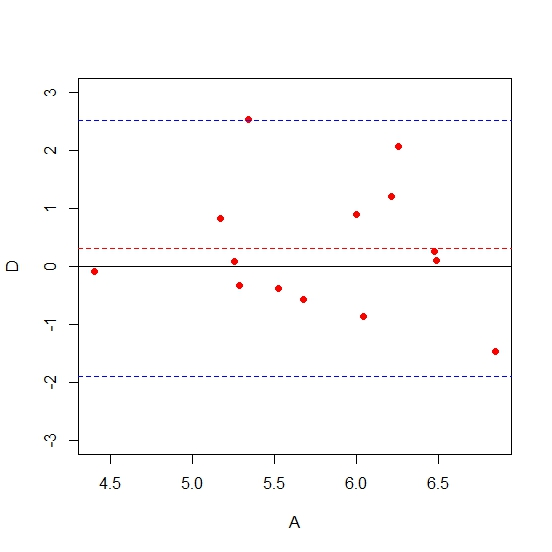
\includegraphics[width=0.6\linewidth]{NewBAplot2}
\label{fig:SimpleBAplot2}
\end{figure}


\end{frame}


\begin{frame}
	\begin{figure}
\centering
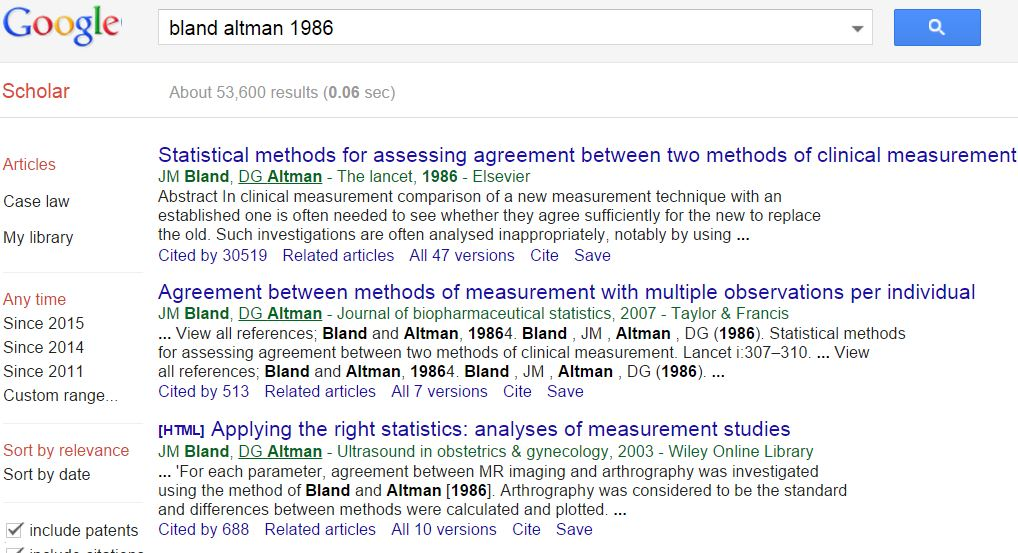
\includegraphics[width=0.9\linewidth]{BACITE}

\label{fig:BACITE}
\end{figure}

\end{frame}
\begin{frame}
	\begin{figure}
		\centering
		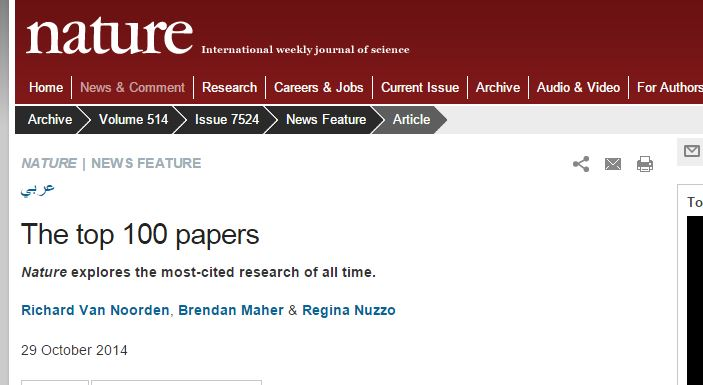
\includegraphics[width=0.9\linewidth]{BACITENATURE}
		
		\label{fig:BACITENATURE}
	\end{figure}
	
\end{frame}
%=================================================================== %
\begin{frame}
	\begin{figure}
		\centering
		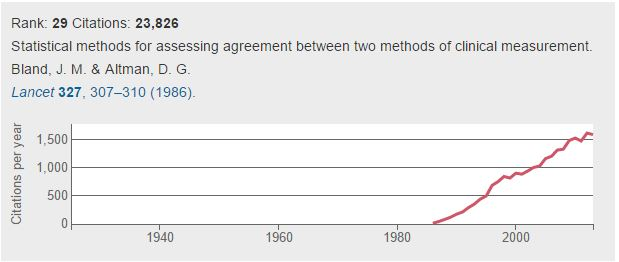
\includegraphics[width=0.99\linewidth]{BACITE1}
		
		\label{fig:BACITE1}
	\end{figure}
	
\end{frame}
%==================================================================== %
\begin{frame}
	\begin{figure}
		\centering
		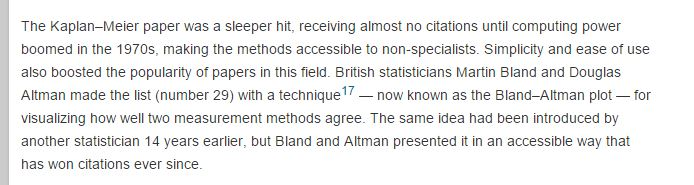
\includegraphics[width=0.99\linewidth]{BACITE2}
		
		\label{fig:BACITE2}
	\end{figure}
	
\end{frame}
%------------------------------------------------------------------------%

\begin{frame}{\bf \tcb{The Bland-Altman Plot: Prevalence}}
\begin{itemize}\itemsep0.7cm

\item Limits of Agreement are used extensively in medical literature for assessing agreement between two methods.
\item Building Blocks are featured in almost every undergraduate statistics course (i.e. Mean, Standard Deviation, Scatterplot, Normal Distribution)
\item Other graphical techniques, such as \textit{Survival-Agreement Plot} (based on Kaplan-Meier Curve) and \textit{Mountain Plot} not prevalent at all.
\end{itemize}
\end{frame}
%========================================================================= %
\section{TAM and SHINY}
\begin{frame}
		\frametitle{Technology Acceptance Model}
	\vspace{-0.4cm}
Davis (1989) proposes the TAM model, which suggests an hypothesis as to why users may adopt particular technologies, and not others. \\ \bigskip
When users are presented with a new 
technology, two important factors will influence their decision about how and when they will adopt it.
\begin{description}
	\item[Perceived usefulness (PU)] - This was defined by Fred Davis as "the degree to which a person believes that using a particular system would enhance his or her job performance".
	\item[Perceived ease-of-use (PEOU)] - Davis defined this as "the degree to which a person believes that using a particular system would be free from effort" 
\end{description}
\end{frame}
%======================================================================= %

\begin{frame}
	\frametitle{Technology Acceptance Model}

\begin{figure}
\centering
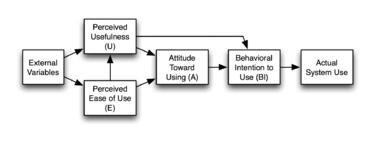
\includegraphics[width=0.79\linewidth]{TechAccept}
\caption{Technology Acceptance Model Flowchart (Davis,1989)}
\label{fig:TechAccept}
\end{figure}

\end{frame}
%====================================================================== %

\begin{frame}
	\Large
	\begin{itemize}
		\item Bland-Altman method not very good on it's own.
		\item Develop a proper methodology for MCS
		
		\item Get people to use it!
	\end{itemize}
\end{frame}

%====================================================================== %
\begin{frame}
	\begin{figure}
\centering

\includegraphics[width=0.99\linewidth]{SHINY}
\end{figure}

\end{frame}
%==================================================================== %

\begin{frame}
\frametitle{Shiny Web Applications with R}
\Large
Useful Shiny Resources

\begin{itemize}
\item  shiny.rstudio.com \bigskip
\item  showmeshiny.com \bigskip
\item  shiny.snap.uaf.edu/ \bigskip
\end{itemize}
\end{frame}

\begin{frame}
	\begin{figure}
		\centering
		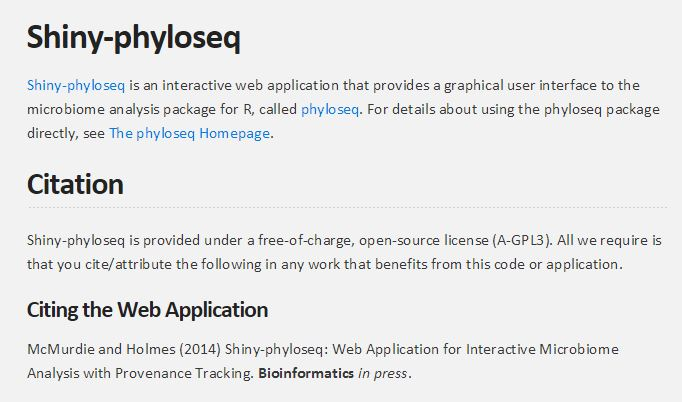
\includegraphics[width=0.99\linewidth]{SHINYCITE}
	\end{figure}
	
\end{frame}
%------------------------------------------------------------------------%

\begin{frame}{\bf \tcb{Replicate Measurements}}
\begin{itemize}\itemsep0.7cm
\item Bland and Altman's approach originally devised for a single measurement on each item by each of the methods.
\item Their 1999 paper \cite{BA99} extended their approach to replicate measurements:\\ \emph{By replicates we mean two or more measurements on the same
individual taken in identical conditions. \\In general this requirement means that the
measurements are taken in quick succession. }
\item Emphasis put on "repeatability".
\end{itemize}
\end{frame}

%------------------------------------------------------------------------%

\begin{frame}{\bf \tcb{Three Conditions}}
For two methods of measurement to be considered interchangeable, the following conditions must apply \cite{Roy2009}:
\\
\begin{itemize}\itemsep0.5cm
\item No significant inter-method bias
\item No difference in the between-subject variabilities of the two methods
\item No difference in the within-subject variabilities of the two methods (repeatability)
\end{itemize}
\end{frame}

\section[Roy's LME Model]{Roy's LME Model}
\subsection{Roy's LME Model}
%------------------------------------------------------------------------%
\begin{frame}{\bf \tcb{LME models}}
\begin{itemize}\itemsep0.7cm
\item In a linear mixed-effects model, responses from a subject are due to both fixed and random
effects. A random effect is an effect associated with a sampling procedure.
\item Replicate measurements would require use of random effect terms in model.
\item Can have differing number of replicate measurements for different subjects.
\end{itemize}
\end{frame}
%------------------------------------------------------------------------%
\begin{frame}{\bf \tcb{Roy's Approach}}
\begin{itemize}\itemsep0.7cm
\item Roy proposes an LME model with Kronecker product covariance structure in a doubly multivariate setup.
\item Response for $i$th subject can be written as
\[ y_i = \beta_0 + \beta_1x_{i1} + \beta_2x_{i2} + b_{1i}z_{i1}  + b_{2i}z_{i2} + \epsilon_i \]
\item $\beta_1$ and $\beta_2$ are fixed effects corresponding to both methods. ($\beta_0$ is the intercept.)
\item $b_{1i}$ and $b_{2i}$ are random effects corresponding to both methods.
\end{itemize}
\end{frame}

%------------------------------------------------------------------------%
\begin{frame}{\bf \tcb{Roy's LME model}}
\begin{itemize}\itemsep0.7cm

\item Let $\boldsymbol{y}_i$ be the set of responses for subject $i$ ( in matrix form).
\item $\boldsymbol{y}_i = \boldsymbol{X}_i\boldsymbol{\beta} + \boldsymbol{Z}_i \boldsymbol{b}_i + \boldsymbol{\epsilon}_i$
\item $\boldsymbol{b}_i \sim N_m(0,\boldsymbol{D})$  (m: number of methods)
\item $\boldsymbol{\epsilon}_i \sim N_{n_i}(0,\boldsymbol{R})$ ($n_i$: number of measurements on subject $i$)
\end{itemize}
\end{frame}

%------------------------------------------------------------------------%


\begin{frame}{\bf \tcb{Variance-covariance matrix}}
\begin{itemize}
\item Overall variance covariance matrix for response vector $\boldsymbol{y}_i$

\[ \mbox{Cov}(\boldsymbol{y}_i)= \boldsymbol{Z}_i \boldsymbol{D}\boldsymbol{Z}^{\prime}_i + \boldsymbol{R}_i \]

\item can be re-expressed as follows:
\[\boldsymbol{Z}_i \left[ \begin{array}{cc} d^2_1 & d_{12}\\
d_{12} & d^2_2\\ \end{array}\right]\boldsymbol{Z}^{\prime}_i  +  \left(V \otimes \left[\begin{array}{cc} \sigma^2_1 & \sigma_{12}\\
\sigma_{12} & \sigma^2_2\\ \end{array}\right] \right)
\]

\item Overall variability between the two methods is sum of between-subject and within-subject variability,
\[
 \mbox{Block } \boldsymbol{\Omega}_i = \left[ \begin{array}{cc} d^2_1 & d_{12}\\ d_{12} & d^2_2\\ \end{array} \right]
+ \left[\begin{array}{cc} \sigma^2_1 & \sigma_{12}\\ \sigma_{12} & \sigma^2_2\\ \end{array}\right].
\]

\end{itemize}
\end{frame}



\section[Implementation]{Implementation}
\subsection{Implementation}

\begin{frame}{\bf \tcb{Variance-Covariance Structures}}
\[\left(
\begin{array}{cc}
\sigma^2_1 & \sigma_{12}\\
\sigma_{12} & \sigma^2_2\\
\end{array} \right)
\]

\begin{itemize}
\item Symmetric structure specifies that $\sigma^2_1$ may differ from $\sigma^2_2$.
\item Compound symmetric structure specifies that $\sigma^2_1 = \sigma^2_2$.
\item In both cases, $\sigma_{12}$ may take value other than 0.
\end{itemize}

\end{frame}
%------------------------------------------------------------------------%
\begin{frame}{\bf \tcb{The \texttt{nlme} Package}}

\begin{itemize}
\item LME models can be implemented in \texttt{R} using the \texttt{nlme} package, one of the core packages.\\
\item Authors: Jose Pinheiro, Douglas Bates (up to 2007), Saikat
DebRoy (up to 2002), Deepayan Sarkar (up to 2005), the \texttt{R} Core team \\(source: \texttt{nlme} package manual)\\
\item ``Mixed-Effects Models in S and S-PLUS" by JC Pinheiro and DM Bates (Springer,2000)

\end{itemize}

\end{frame}
%------------------------------------------------------------------------%
\begin{frame}[fragile]{\bf \tcb{The Reference Model}}
\texttt{REF = lme(y $\sim$ meth,\\
   \hspace{0.6cm} data = dat,\\
   \hspace{0.6cm} random = list(item=\tcr{pdSymm}($\sim$ meth-1)), \\
   \hspace{0.6cm} weights=varIdent(form=$\sim$1|meth),\\
   \hspace{0.6cm} correlation = \tcr{corSymm}(form=$\sim$1 | item/repl),\\
   \hspace{0.6cm} method="ML")}\\
\begin{itemize}
\item LME model that specifies a symmetric matrix structure for both between-subject and within-subject variances.
\end{itemize}

\end{frame}

%------------------------------------------------------------------------%
\begin{frame}[fragile]{\bf \tcb{The Nested Model 1}}
\texttt{NMB = lme(y $\sim$ meth,\\
   \hspace{0.6cm} data = dat,\\
   \hspace{0.6cm} random = list(item=\tcr{pdCompSymm}($\sim$ meth-1)), \\
   \hspace{0.6cm} weights=varIdent(form=$\sim$1|meth),\\
   \hspace{0.6cm} correlation = \tcr{corSymm}(form=$\sim$1 | item/repl),\\
   \hspace{0.6cm} method="ML")}

\begin{itemize}
\item LME model that specifies a compound symmetric matrix structure for between-subject and symmetric structure within-subject variances.
\end{itemize}

\end{frame}
%------------------------------------------------------------------------%
\begin{frame}[fragile]{\bf \tcb{The Nested Model 2}}
\texttt{NMW = lme(y $\sim$ meth,\\
   \hspace{0.6cm} data = dat,\\
   \hspace{0.6cm} random = list(item=\tcr{pdSymm}($\sim$ meth-1)), \\
   \hspace{0.6cm} \tcb{\#weights=varIdent(form=$\sim$1|meth),}\\
   \hspace{0.6cm} correlation = \tcr{corCompSymm}(form=$\sim$1 | item/repl),\\
   \hspace{0.6cm} method="ML")}
   \begin{itemize}
\item LME model that specifies a symmetric matrix structure for between-subject and compound symmetric structure within-subject variances.
\end{itemize}
\end{frame}
%------------------------------------------------------------------------%

\begin{frame}[fragile]{\bf \tcb{The Nested Model 3}}
\texttt{NMO = lme(y $\sim$ meth,\\
   \hspace{0.6cm} data = dat,\\
   \hspace{0.6cm} random = list(item=\tcr{pdCompSymm}($\sim$ meth-1)), \\
   \hspace{0.6cm} \tcb{\#weights=varIdent(form=$\sim$1|meth),}\\
   \hspace{0.6cm} correlation = \tcr{corCompSymm}(form=$\sim$1 | /repl),\\
   \hspace{0.6cm} method="ML")}
   \begin{itemize}
\item LME model that specifies a compound symmetric matrix structure for both between-subject and within-subject variances.
\end{itemize}
\end{frame}



%------------------------------------------------------------------------%
\section[Example]{Example}
\subsection{Example}
\begin{frame}{\bf \tcb{Example: Blood Data}}
\begin{itemize}\itemsep0.7cm
\item Used in Bland and Altman's 1999 paper \cite{BA99}. Data was supplied by Dr E O'Brien.
\item Simultaneous measurements of systolic blood pressure each made by two experienced observers, J and R, using a  sphygmometer.
\item Measurements also made by a semi-automatic blood pressure monitor, denoted S.
\item On 85 patients, 3 measurement made in quick succession by each of the three observers (765 measurements in total)
\end{itemize}
\end{frame}
%------------------------------------------------------------------------%

\begin{frame}[fragile]{\bf \tcb{Example: Blood Data}}
Inter-method Bias between J and S:         15.62 mmHg
\begin{verbatim}
>summary(REF)
.....
Fixed effects: y ~ meth
             Value Std.Error  DF t-value p-value
(Intercept) 127.41    3.3257 424  38.310       0
methS        15.62    2.0456 424   7.636       0
.....
\end{verbatim}
\end{frame}
%------------------------------------------------------------------------%

\begin{frame}[fragile]{\bf \tcb{Between-subject variance covariance matrix }}

\begin{verbatim}
..
Random effects:
 Formula: ~method - 1 | subject
 Structure: General positive-definite
         StdDev    Corr
methodJ  30.396975 methdJ
methodS  31.165565 0.829
Residual  6.116251
..
\end{verbatim}
\[
\hat{\boldsymbol{D}} = \left(
\begin{array}{cc}
923.97	& 785.34 \\
785.34	& 971.29\\
\end{array}\right)
\]
\end{frame}

%------------------------------------------------------------------------%
\begin{frame}[fragile]{\bf \tcb{Within-subject variance covariance matrix}}
\begin{verbatim}
Correlation Structure: General
 Formula: ~1 | subject/obs
 Parameter estimate(s):
 Correlation:
  1
2 0.288
Variance function:
 Structure: Different standard deviations per stratum
 Formula: ~1 | method
 Parameter estimates:
       J        S
1.000000 1.490806
\end{verbatim}
\[
 \hat{\boldsymbol{\Sigma}} = \left(
\begin{array}{cc}
37.40 & 16.06 \\
16.06 & 83.14 \\
\end{array}\right)
\]
\end{frame}
%------------------------------------------------------------------------%
\begin{frame}[fragile]{\bf \tcb{Overall variance covariance matrix}}

\begin{itemize}\itemsep0.7cm
\item Overall variance \[
\mbox{Block }\hat{\boldsymbol{\Omega}} = \hat{\boldsymbol{D}} + \hat{\boldsymbol{\Sigma}} =
 \left(
\begin{array}{cc}
961.38 & 801.40 \\
801.40 & 1054.43 \\
\end{array}
\right)
\]

\item Standard deviation of the differences can be computed accordingly : 20.32 mmHg.

\item Furthermore, limits of agreement can be computed: $[15.62 \pm (2 \times 20.32) ]$ (mmHg).
\end{itemize}
\end{frame}

%------------------------------------------------------------------------%

\begin{frame}{\bf \tcb{Some useful \texttt{R} commands}}
\begin{itemize}

\item \texttt{intervals} :\vspace{0.25cm} \\This command obtains the estimate and confidence intervals on the parameters associated with the model.\\
    This is particularly useful in writing some code to extract estimates for inter-method bias and variances, and hence estimates for the limits of agreement.

\item \texttt{anova} : \vspace{0.25cm} \\When a reference model and nested model are specified as arguments, this command performs a likelihood ratio test.
\end{itemize}
\end{frame}


%------------------------------------------------------------------------%
\begin{frame}[fragile]{\bf \tcb{Formal Tests: Between-subject Variances}}
\begin{itemize}
\item Test the hypothesis that both methods have equal between-subject variances.
\item Constructed an alternative model ``Nested Model B" using \textbf{\emph{compound symmetric}} form for between-subject variance (hence specifying equality of between-subject variances).
\item Use a likelihood ratio test to compare models.
\end{itemize}
\begin{verbatim}
...
> anova(REF,NMB)
   Model df ...     logLik   Test   L.Ratio p-value
REF    1  8 ...  -2030.736
NMB    2  7 ...  -2030.812 1 vs 2 0.1529142  0.6958
...
\end{verbatim}
\begin{itemize}
\item Fail to reject hypothesis of equality.
\end{itemize}
\end{frame}

%------------------------------------------------------------------------%
\begin{frame}[fragile]{\bf \tcb{Formal Tests: Within-subject Variances}}
\begin{itemize}
\item Test the hypothesis that both methods have equal within-subject variances.
\item Constructed an alternative model ``Nested Model W" using compound symmetric form for within-subject variance (hence specifying equality of within-subject variances).
\item Again, use a likelihood ratio test to compare models.
\end{itemize}
\begin{verbatim}
...
> anova(REF,NMW)
    Model df ...    logLik   Test  L.Ratio p-value
REF     1  8 ... -2030.736
NMW     2  7 ... -2045.044 1 vs 2 28.61679  <.0001
\end{verbatim}
\begin{itemize}
\item Reject hypothesis of equality.
\end{itemize}
\end{frame}
%------------------------------------------------------------------------%
\begin{frame}[fragile]{\bf \tcb{Formal Tests : Outcomes}}
\begin{itemize}
\item Inter-method bias: Significant difference in mean values detected.\\
\vspace{0.25cm}\item Between-subject variance: No significant difference in between-subject variances between the two methods detected.\\
\vspace{0.25cm}\item Within-subject variance: A significant difference in within-subject variances is detected.\\
\vspace{0.25cm}\item Can not recommend switching between the two methods.
\end{itemize}
\end{frame}
%------------------------------------------------------------------------%
\begin{frame}[fragile]{\bf \tcb{Remarks}}
\begin{itemize}
\item Can perform a test for equality of overall variances.\\
\vspace{0.25cm}\item This can be done by specifying a compound symmetry structure for both between-subject and within-subject variances when constructing a nested model.\\
\vspace{0.25cm}\item Roy controls the family-wise error rate in paper, using Bonferroni correction procedure.
\end{itemize}
\end{frame}
%------------------------------------------------------------------------%
\section[References]{References}
\subsection{References}
\begin{frame}{\bf \tcb{References}}
\begin{thebibliography}{99}
\bibitem{Roy2009} A Roy (2009): \emph{An application of linear mixed effects model to assess the agreement between two methods with replicated observations} Journal of Biopharmaceutical Statistics
\bibitem{BA86} Bland JM, Altman DG (1986) \emph{Statistical method for assessing agreement between two methods of clinical measurement}.
\bibitem{BA99} Bland JM, Altman DG (1999)  \emph{Measuring agreement in method comparison studies.} Statistical Methods in Medical Research
\bibitem{PB} Pinheiro JC, Bates DM (2000): \emph{Mixed-effects models in S and S-PLUS},
Springer.
%\bibitem{BXC2008} B Carstensen, J Simpson, and LC Gurrin (2008): \emph{ Statistical models for assessing agreement in method comparison studies with replicate measurements.} International Journal of Biostatistics.
\end{thebibliography}
\end{frame}

%------------------------------------------------------------------------%

\begin{frame}{\bf \tcb{Thanks}}
\begin{itemize}
\item Dr Kevin Hayes, University of Limerick
\item Dr Kevin Burke, University of Limerick
\item Peter Fennell
\end{itemize}
\end{frame}


\end{document} 